We consider a N sites one dimensional wire connected to two semi-infinite leads. We model the system by the following tight-binding Hamiltonian:
\begin{equation}
\textbf{H} = -\gamma \sum_{i}c^{\dagger}_i c_{i+1} + \sum_{i} w(t)\theta(-i) c^{\dagger}_i c_{i} + \sum_{i} V_{QPC}(i) c^{\dagger}_i c_{i}
\end{equation}
The scattering region will be indexed by $i \in [\![1,N]\!]$, whereas left (right) lead sites are indexed with $i \leq 0$
 ($i \geq N+1$). The hopping  The voltage pulse is modeled by the second term, with $\theta(x)$ being the Heaviside function and $w(t)$:
 \begin{equation}
 	w(t) = V_P e^{-2(\frac{t-t_0}{\tau})^2}
 \end{equation}
 $V_P$ being the amplitude, $\tau$ the width and $t_0$ the starting time of the perturbation. We introduced a Quantum Point Contact (QPC) which consists in a filtering potential barrier:
 \begin{equation}
V_{QPC}(i) = V_0 e^{-(\frac{i - i_0}{\xi})^2}
 \end{equation}
 $V_0$ being the amplitude, $\xi$ the width and $x_0$ the position of the QPC.
 The time-dependent peturbation can be absorbed by the gauge transforming leading to a redefinition of the hopping parameter the left lead where the pulse is applied and the scattering region:
 \begin{equation}
\gamma \rightarrow \gamma e^{-i\phi(t)}
 \end{equation}
 with:
 \begin{equation}
 	\phi(t) = \frac{e}{\hbar}\int_{-\infty}^{t} w(u)du
 \end{equation}
 
\begin{figure}[h]
	\centering
	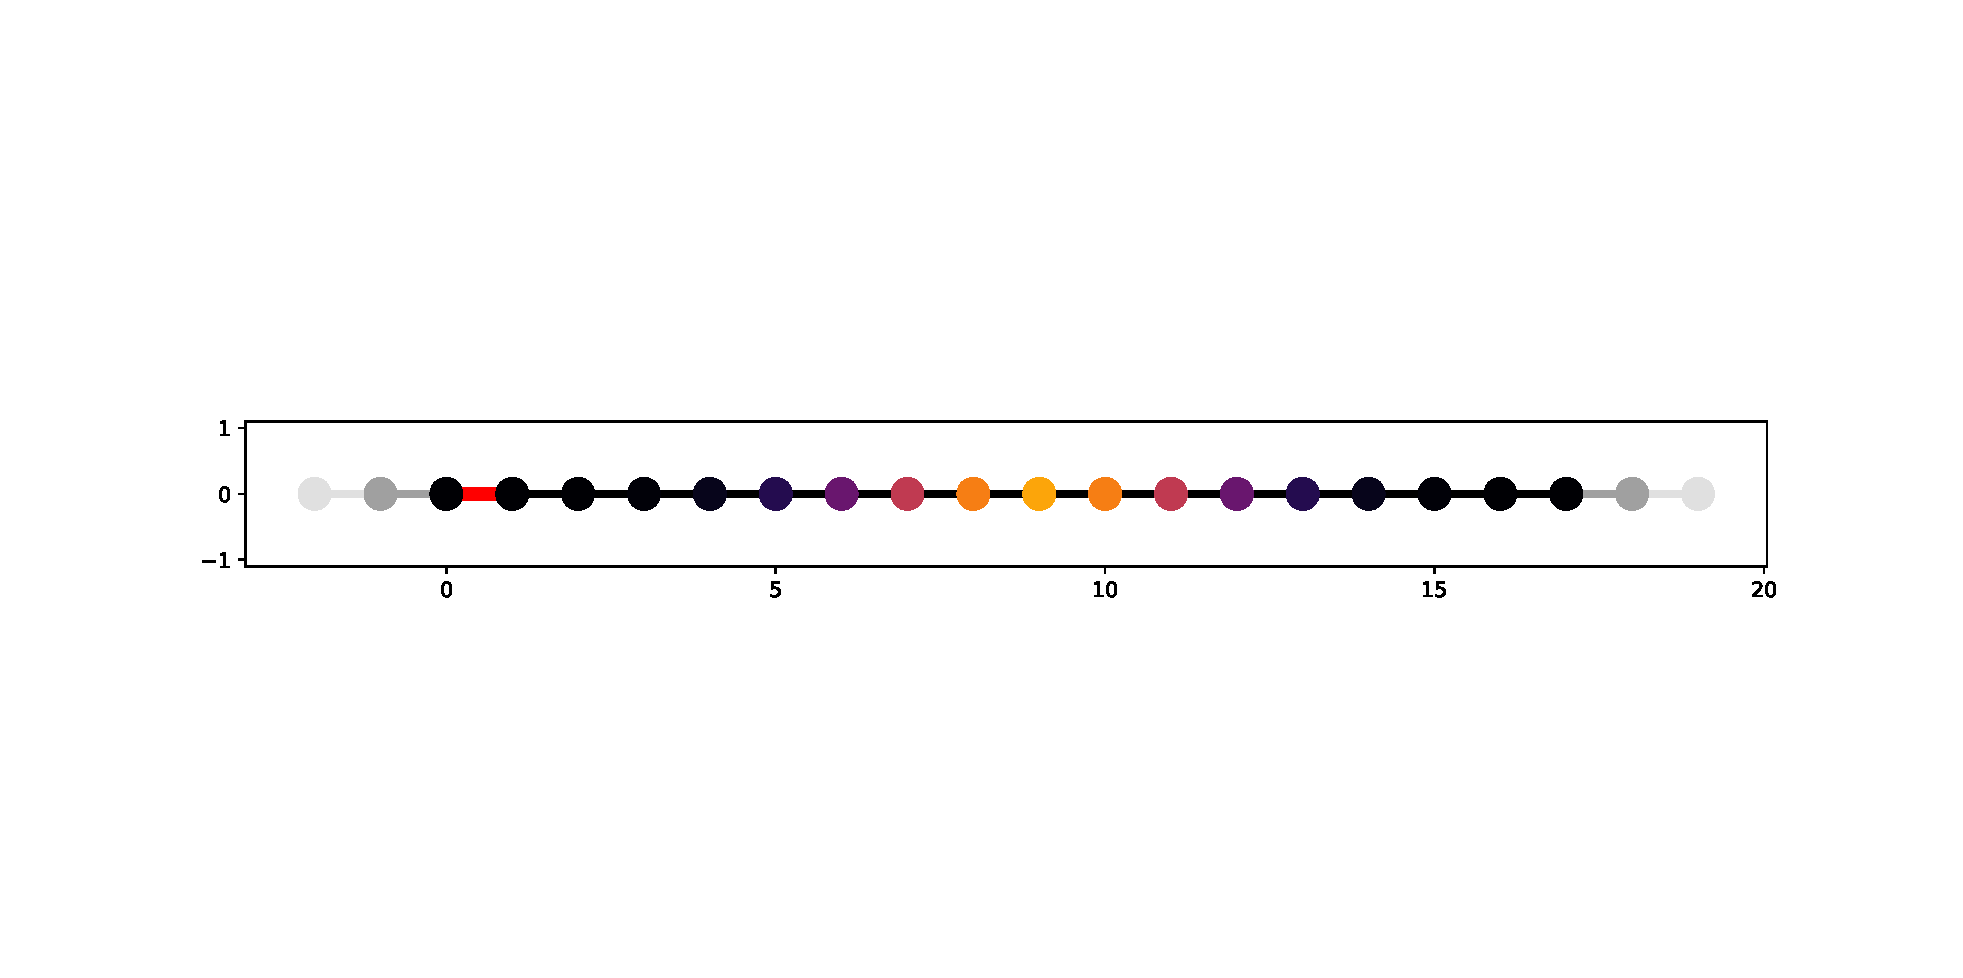
\includegraphics[width = 0.6\linewidth]{../figures/syst_color}
	\caption{A schematic of the system. The wire is connected to two semi-infinte leads. The site color reflects the QPC's voltage amplitude. The time-dependent hopping parameter is displayed in red. }
	\label{fig:systcolor}
\end{figure}